\epigraph{``Since Newton, mankind has come to realise that the law of physics are always expressed in the language of differential equations"}{Steven Strogatz}

\section{Finite Difference Method}\label{fdm_section}
\subsection{Introduction}
The use of numerical models for the simulation of dynamics within the atmosphere typically involves the solution of a set of partial differential equations. These equations generally describe three processes: advection, adjustment and diffusion. 

\begin{definition}
Advection is the transport of a substance by bulk motion.
\end{definition}

\begin{definition}
Adjustment is how the mass and wind fields adjust to one another.
\end{definition}

\begin{definition}
Diffusion is the movement of a liquid, or gas from an area of high concentration to an area of low concentration.
\end{definition}

Most meteorological problems involving partial differential equations generally fall into three distinct categories: initial value problems, boundary value problems, and eigenvalue problems. The meteorological problems associated with this project are solely initial value problems\cite{numerical_methods}. An initial value problem is a situation where you want to predict the future state of a given system, given the necessary initial conditions. Unfortunately, the equations describing the evolution of the atmosphere do not have exact analytical solutions.

\begin{definition}
An analytical function is the most precise way of representing a  physical field as it gives us the value of this field at any point in space, and at any instant in time.
\end{definition}

When an analytical solution does not exist, an approximate numerical solution is found using a specified computational technique\cite{numerical_methods}. For the purposes of this project, the finite difference method will be utilised. It must be noted, however, that there are several other methods to acquire an approximate numerical solution, with the finite element method and the spectral method being just a few.

The idea of the finite difference method is to approximate the derivatives in the partial differential equations with differences between adjacent points in space and in time. The advantages of this being that the problem becomes an algebraic one, and that a continuous problem becomes a discrete one.

\subsection{Derivation of the Finite Difference Method}

In order to derive the finite difference method, it is necessary to look at the Taylor series expansion of the function.

\begin{definition}
The Taylor series of a function is the limit of that function's Taylor polynomials as the degree increases.
\end{definition}

The Taylor series expansion of $f(x)$ can be represented as the following:

\begin{equation}
    f(x + \Delta x) = f(x) + \frac{d f}{d x}(x) \frac{\Delta x}{1!} + \frac{d^2 f}{d x^2}(x) \frac{\Delta x^2}{2!} + ... + \frac{d^n f}{d x^n}(x) \frac{\Delta x^n}{n!} + ...
\end{equation}
\begin{equation}
    f(x - \Delta x) = f(x) + \frac{d f}{d x}(x) \frac{-\Delta x}{1!} + \frac{d^2 f}{d x^2}(x) \frac{(-\Delta x)^2}{2!} + ... + \frac{d^n f}{d x^n}(x) \frac{(-\Delta x)^n}{n!} + ...
\end{equation}

The higher order terms, which will be represented as $\mathcal{O}(\Delta x)$ from this point on, become less important as $\Delta x$ approaches zero.

\begin{equation}
    \Rightarrow f(x + \Delta x) = f(x) + \frac{d f}{d x}(x) \frac{\Delta x}{1!} + \frac{d^2 f}{d x^2}(x) \frac{\Delta x^2}{2!} + [\mathcal{O}(\Delta x^3)] 
    \label{fds}
\end{equation}
\begin{equation}
    \Rightarrow f(x - \Delta x) = f(x) - \frac{d f}{d x}(x) \frac{\Delta x}{1!} + \frac{d^2 f}{d x^2}(x) \frac{\Delta x^2}{2!} + [\mathcal{O}(\Delta x^3)]
    \label{bds}
\end{equation}

These higher order terms are neglected, and the following approximation for the derivative of $f(x)$ is found:

\begin{equation}
    \Rightarrow \frac{d f}{d x}(x) = \frac{f(x + \Delta x) - f(x)}{\Delta x} + \mathcal{O}(\Delta x)
\end{equation}
\begin{equation}
    \Rightarrow \frac{d f}{d x}(x) = \frac{f(x - \Delta x) - f(x)}{\Delta x} + \mathcal{O}(\Delta x)
\end{equation}

These are called the forward and backward difference schemes respectively, and by keeping only the leading order terms, an error of order $\mathcal{O}(\Delta x)$ is occurred. It is possible to obtain a better approximation by subtracting \ref{bds} from \ref{fds}, which yields equation \ref{eq_fds_bds_subtract}.

\begin{equation}
    \frac{d f}{d x}(x) = \frac{f(x + \Delta x) - f(x - \Delta x)}{\Delta x} + \mathcal{O}(\Delta x^2)
    \label{eq_fds_bds_subtract}
\end{equation}

This particular approximation is called the central difference scheme, and has an error of order $\mathcal{O}(\Delta x^2)$. Therefore, this scheme is more accurate than the previously mentioned forward and backward difference schemes. It is possible to take more and more terms from the Taylor series expansion, however, there is an inherent trade off between accuracy and computational efficiency. 

In relation to the atmosphere, what this method does is divide the atmosphere into several discrete horizontal layers, and each layer is divided up into grid cells. Following which, each equation is evaluated at the centre of the cell. Similarly, the time interval under consideration is sliced into a number of discrete time steps. The size of the grid step $\Delta x$ and time step $\Delta t$ determines the accuracy of the scheme, with accuracy increasing as $\Delta x$ and $\Delta t$ approach zero. On a synoptic scale, $\Delta x$ is generally equal to 500 km. For higher resolutions, the grid-size is smaller, which corresponds to a greater computational burden. As such, there is a trade off between accuracy and computational performance. For Eulerian schemes, the typical time step is 2 minutes. As such, since the software will use an Eulerian scheme, the time step will be 2 minutes\cite{leapfrog_slides_one}.

\subsection{FTCS Scheme}\label{ftcs_section}

Given the information mentioned in the previous section, the most obvious scheme to approximate a differential equation, which will be used to predict the future state of the atmosphere, would be to combine the central difference scheme for space and the forward difference scheme for time (FTCS). This scheme would allow us access to the increased accuracy of the central difference scheme, while maintaining two time variable unknowns. If only it was that simple! Let's take the example of the 1-D linear advection equation for temperature. This equation is represented as the following:

\begin{equation}
    \frac{\partial T}{\partial t} + u \frac{\partial T}{\partial x} = 0
    \label{1d_temp_eq}
\end{equation}

Using the FTCS scheme mentioned above, this equation can be approximated as:

\begin{equation}
    \frac{T^{n+1}_{i} - T^{n}_{i}}{\Delta t} + u \frac{T^{n}_{i+1} - T^{n}_{i-1}}{2 \Delta x} = 0
\end{equation}

It can be shown, by using Fourier Series, that:

\begin{equation}
    |\lambda_j|^2 = 1 + \alpha^2(\sin{j \Delta x}^2)
\end{equation}

Therefore, $|\lambda_j|^2 \geq 1$, and so the scheme is said to be absolutely unstable. What it means for a scheme to be unstable is that if there is a slight change in the initial value, the result of the computation will change dramatically. The stability of a scheme is important in meteorological problems because if slight deviations from the mathematical model caused by unavoidable errors in measurement do not have a correspondingly slight effect on the approximate numerical solution, the mathematical equations describing the problem will not accurately predict the future outcome\cite{ftcs_leapfrog}. For a more detailed technical explanation of the stability of this scheme and the leapfrog scheme (discussed in section \ref{leapfrog}), please see the following article: \url{https://www.ecmwf.int/sites/default/files/elibrary/2002/16948-numerical-methods.pdf}.

\subsection{Leapfrog Scheme}\label{leapfrog}

This scheme is probably the most common scheme used for meteorological problems. The "leapfrog" refers to the centred
time difference which is used in conjunction with centred space differences. 

Taking the 1-D linear advection equation for temperature seen in equation \ref{1d_temp_eq}, applying this scheme results in:

\begin{equation}
    \frac{T^{n+1}_{i} - T^{n-1}_{i}}{2 \Delta t} + u \frac{T^{n}_{i+1} - T^{n}_{i-1}}{2 \Delta x} = 0
\end{equation}

It can be shown that this scheme is stable using a similar technique mentioned in section \ref{ftcs_section}. This equation can then be rearranged for the forecast value $T^{n+1}_{i}$\cite{ftcs_leapfrog}:

\begin{equation}
    T^{n+1}_{i} = T^{n-1}_{i} - u \frac{2 \Delta t}{2 \Delta x}(T^{n}_{i+1} - T^{n}_{i-1})
\end{equation}

For the physical equation, a single initial condition $T^{0}$ is sufficient to determine the solution. One problem with the leapfrog scheme is that two values of $T$ are required to start the computation. In addition to the physical initial condition $T^{0}$, a computational initial condition $T^{1}$ is required. This cannot be obtained using the leapfrog scheme, so a non-centred step is used to provide the value at $t = \Delta t$. From which point on, the leapfrog scheme is used, however, the errors of the first step will persist. This method, however, still retains an error of order $\mathcal{O}(\Delta t^2)$. If you also use half of the time step for the forward time step, followed by leapfrog time steps; this will reduce the error introduced in the first step\cite{leapfrog_slides_two}. This will be the method utilised within the software.

\subsection{Nonlinear Instability}
A major problem which occurs while dealing with nonlinear partial differential equations is nonlinear instability. This is a problem where there is a nonlinear interaction between atmospheric waves\cite{nonlinear_instability}.  

\begin{definition}
An atmospheric wave is a periodic disturbance in the fields of atmospheric variables (like geopotential height, temperature, or wind velocity) which may either propagate (travelling wave) or not (standing wave).
\end{definition}

If one of the waves involved in this nonlinear interaction have a wavelength less than $4 \Delta x$ something called aliasing causes a channelling of energy towards the small wavelengths. The continuous feedback of energy leads to a catastrophic rise in the kinetic energy of wavelengths between $2 \Delta x$ and $4 \Delta x$. Within the software, a smoothing operator, which reduces the amplitude of the short waves while having little effect on the meteorologically important waves, is utilised\cite{nonlinear_instability}.

Another problem to mention before moving on is that for nonlinear equations, the leapfrog scheme has a tendency to increase the amplitude of the computational mode with time This can separate the space dependence between the even and odd time steps. This problem can be rectified by applying a Robert-Asselin Time Filter. After $T^{n+1}$ is obtained a slight time smoothing is applied to $T^{n}$, where $\gamma$ is on the order of 0.1\cite{leapfrog_slides_two}:

\begin{equation}
    T^{n} = T^{n} + \gamma(T^{n+1} - 2 T^{n} + T^{n-1})
\end{equation}

\section{Ensemble Prediction System}
\subsection{Introduction}
Ensemble Prediction Systems (EPS) are numerical weather prediction systems that allow for the estimation of uncertainty in a weather forecast, as well as, providing a better prediction for the future state of the atmosphere. Instead of running a atmospheric dynamical simulation once (this would be regarded as deterministic), the simulation is run many different time with slightly different initial conditions. Due to the high computational resources required to run these simulations, they are often run at half the resolution of an equivalent deterministic simulation. The ensemble prediction system has a control simulation that doesn't have any perturbations to the initial conditions. Each simulation that makes up the system is called an ensemble member\cite{intro_efs}.

\subsection{Advantages of EPS}
\begin{figure}[H]
    \centering
    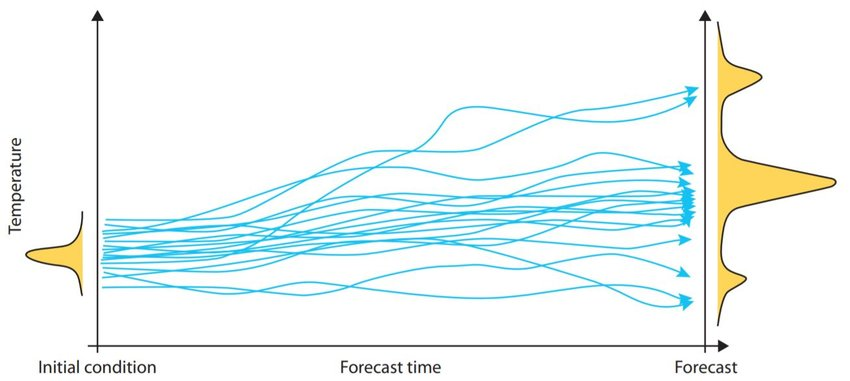
\includegraphics[width=.8\linewidth]{Images/efs.jpg}
    \caption{Visualisation of the Advantages of an Ensemble Prediction System}
    \label{efs}
\end{figure}

As a consequence of Chaos Theory, a tiny difference in the initial conditions in a large system, such as the atmosphere, can result in drastically different forecasted events, so that even with a tiny error, it can become a large error in the forecasted future state of the atmosphere. Even with the most accurate observations, error cannot be avoided. Therefore, it is simply not possible to make a better forecast or simulation. This is why an ensemble prediction system is utilised. In an ensemble simulation, small perturbations are made to the initial conditions, after which, the simulation is re-run. If there is a large degree of overlap between the ensemble members, there will be a higher degree of confidence in the ensemble forecast, with the opposite also holding true\cite{intro_efs}.

\subsection{Global EPS}
There are three distinct types of ensemble prediction systems: global, regional and convective-scale. Each system address different timescales, and different grid-sizes. A global ensemble prediction system is designed and used for medium-range forecasting between 3 and 15 days into the future. They use synoptic simulation models and are run at relatively low resolutions. Although they are primarily designed for use in the medium range, their global coverage means that they can also be used to provide short-range EPS forecasts in regions of the globe where no other EPS are currently available, and may be the only available option for certain countries. Considering the software is focused on synoptic scale simulations, this will be the system of interest\cite{intro_efs}, The default number of ensemble members in the software is fifteen, which is typical for a global ensemble prediction system. The grid-size, used by the software, can be specified by the end-user in order to get a more detailed forecast (this will increase the amount of computational resources required to run the simulation), however, the default grid-size is of the scale of 1000 km. There is also a hard limit of a $5^{\circ} \times 5^{\circ}$ cell, as a smaller cell size would result in inaccurate simulations due to the fact that the dynamical equations utilised by the software do not work on this scale. This will be discussed at greater depth in chapter \ref{4}.

\section{Recurrent Neural Network}
\subsection{Introduction}
Weather forecasting has traditionally been done by physical models of the atmosphere, which are unstable to perturbations, and thus are inaccurate for large periods of time\cite{why_rnn}. Since machine learning techniques are more robust to perturbations, it would be logical to combine a neural network with a physical model. Weather forecasting is a sequential data problem, therefore, a recurrent neural network is the most suitable option for this task. 

\begin{definition}
A recurrent neural network is a class of artificial neural networks where connections between nodes form a directed graph along a temporal sequence.
\end{definition}

Before, we delve into the specific example of using a recurrent neural network to predict the future state of the atmosphere, it is necessary to review what a recurrent neural network is. Recurrent Neural Networks (RNNs) are neural networks that are used in situations where data is presented in a sequence. For example, let's say you want to predict the future position of a fast-moving ball. Without information on the previous position of the ball, it is only possible to make an inaccurate guess. If you had, however, a large number of snapshots of the previous position, you are then able to predict the future position of the ball with some certainty. RNNs excel at modelling sequential data such as these. This is due to sequential memory.

In order to intuitively understand sequential memory, the prime example would be the alphabet. While it is easy to say the alphabet from A-Z, it is much harder to go from Z-A. There is a logical reason why this is difficult. As a child, you learn the alphabet in a sequence. Sequential memory is a mechanism that makes it easier for your brain to recognise sequence patterns.

In a traditional neural network, there is a input layer, hidden layer, and a output layer. In a recurrent neural network, a loop is added that can be added to pass information forward as seen in the diagram below (provided by Towards Data Science)\cite{intro_rnn}:

\begin{figure}[H]
    \centering
    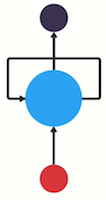
\includegraphics[width=.2\linewidth]{Images/rnn.png}
    \caption{Visualisation of a Recurrent Neural Network}
\end{figure}

The information that is forwarded is the hidden layer, which is a representation of previous inputs. How this works in practise is that you initialise your network layers and the hidden the initial hidden state. The shape and dimension of the hidden state will be dependent on the shape and dimension of your recurrent neural network. Then you loop through your inputs, pass the relevant parameter and hidden state into the RNN. The RNN returns the output and a modified hidden state. Last you pass the output to the output layer, and it returns a prediction. 

There is, however, a major problem known as short-term memory. Short-term memory is caused by something known as the vanishing gradient problem, which is also prevalent in other neural network architectures. As the RNN processes more steps, it has troubles retaining information from previous steps. Short-Term memory and the vanishing gradient is due to the nature of back-propagation. This can be comprehended through understanding how a neural network is trained\cite{intro_rnn}.

\begin{definition}
Back-propagation is an algorithm used to train and optimise neural networks.
\end{definition}

To train a recurrent neural network, you use an application of back-propagation called back-propagation through time. Training a neural network has three major steps. First, the relevant data vector is normalised between 0 and 1, the vector is feed into the RNN, and it goes through an activation function. The activation function utilised in the software is the rectified linear activation function\cite{lstm_rnn}. 

\begin{definition}
The rectified linear activation function is a piece-wise linear function that will output the input directly if is positive, otherwise, it will output zero.
\end{definition}

The function is linear for values greater than zero, meaning it has a lot of the desirable properties of a linear activation function when training a neural network using back-propagation. Yet, it is a nonlinear function as negative values are always output as zero. As a result, the rectified function is linear for half of the input domain and nonlinear for the other half, it is referred to as a piece-wise linear function\cite{relu}. This nonlinear element is extremely important if the system has a nonlinear component, for example in predicting the evolution of the future state of the atmosphere.

\begin{figure}[H]
    \centering
    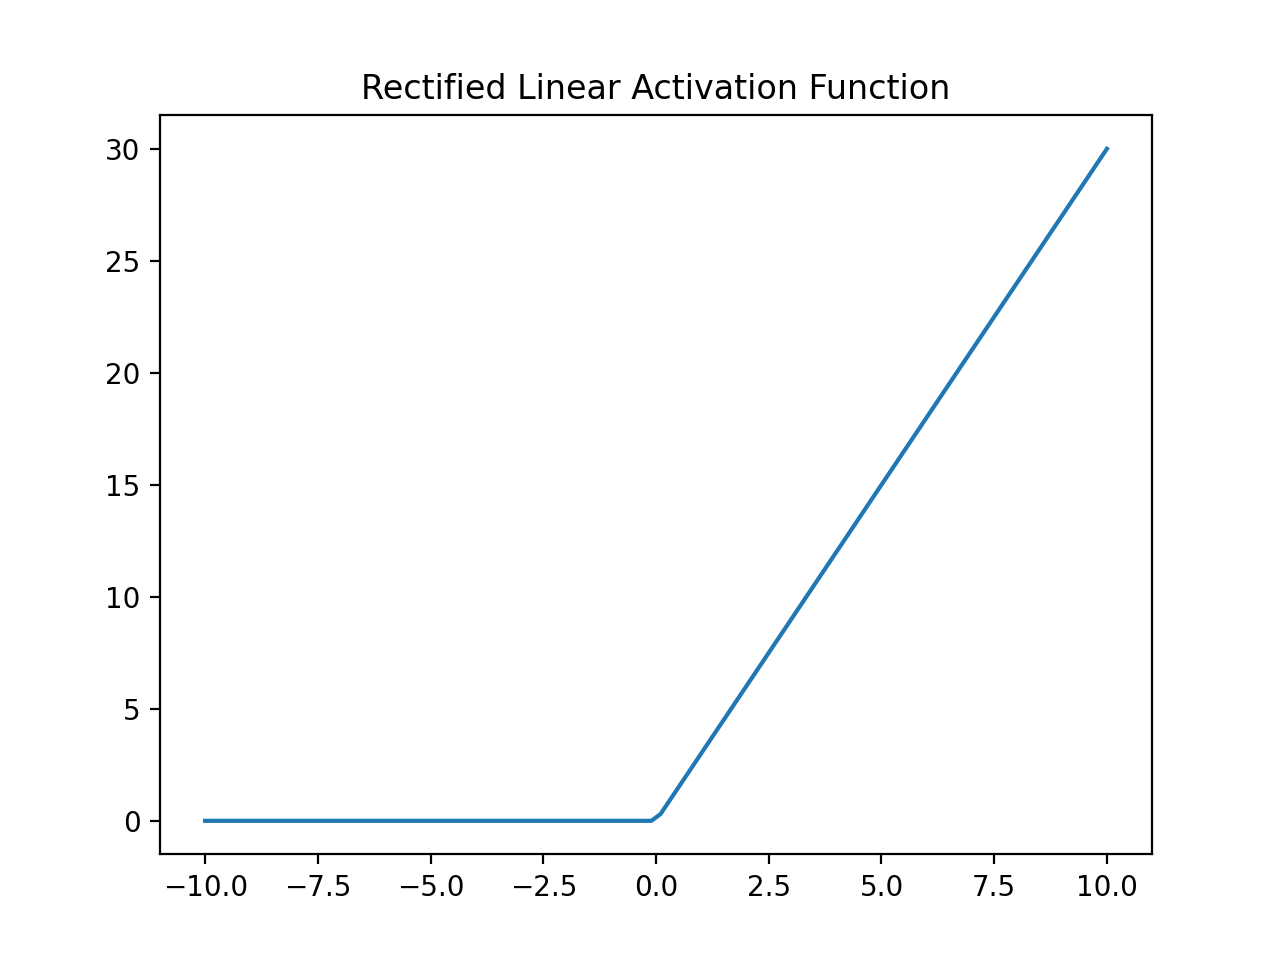
\includegraphics[width=.65\linewidth]{Images/relu.png}
    \caption{Sketch of the Rectified Linear Activation Function}
\end{figure}

Second, it outputs the results. Third, it compares the prediction to the ground truth using a loss function.

\begin{definition}
A loss function outputs an error value which is an estimate of how poorly the network is performing.
\end{definition}

The lost function that will be utilised in the software will be the function for mean squared error. The reason for choosing this particular function is that it heavily penalises large errors, as it squares the difference between the predicted and actual value. A large error in a weather forecast is highly undesirable, hence, the use of this function. The function is represented below:

\begin{equation}
    MSE = \frac{1}{n}\sum_{i=1}^n(Y_i-\hat{Y_i})^2
\end{equation}

If  a vector of $n$ predictions is generated from a sample of $n$ data points on all variables, and $Y$ is the vector of observed values of the variable being predicted, with $\hat{Y_i}$ being the predicted values.

\begin{definition}
Mean squared error is the average squared difference between the estimated values and the actual value.
\end{definition}

Returning to the training of the RNN, it uses that error value from the loss function. to do back propagation which calculates the gradients for each time step in the network. The gradient is the value used to adjust the networks internal weights, allowing the network to learn. The bigger the gradient, the bigger the adjustments and vice versa. Here is where the problem lies. When doing back propagation, the gradient of the current time step is calculated with respect to the effects of the gradients, in the time step before it. So if the adjustments to the time step before it is small, then adjustments to the current time step will be even smaller.  The gradient values will exponentially shrink as it propagates through each time step. That causes gradients to exponentially shrink as it back propagates down. The earlier layers fail to do any learning as the internal weights are barely being adjusted due to extremely small gradients.

Because of vanishing gradients, the RNN doesn’t learn the long-range dependencies across time steps. So not being able to learn on earlier time steps causes the network to have a short-term memory. In order to combat this, a long short-term memory is used\cite{intro_rnn}.

\subsection{LSTM}
LSTM's were created as a solution to the short-term memory problem. They have internal mechanisms called gates that can regulate the flow of information. These gates can learn which data in a sequence is important to keep or throw away. By doing that, it can pass relevant information down the long chain of sequences to make predictions. For example, if you were interested in buying a particular, you might read a review in order to determine if the purchase of the product is a good decision. When you read a review, your brain subconsciously only remembers important keywords. You pick up words like ``amazing", ``superb", or ``awful", you don't remember words such as "the", "as", or "because". This is what an LSTM does, it learns to keep only the relevant information to make predictions.

An LSTM has a similar control flow as a recurrent neural network. It processes data passing on information as it propagates forward. The differences are the operations within the LSTM’s cells. The core concept of LSTM’s are the cell state, and it’s various gates. The cell state is the method by which information is transferred down the sequence chain. The cell state, in theory, can carry relevant information throughout the processing of the sequence. So even information from the earlier time steps can make it’s way to later time steps, reducing the effects of short-term memory. As the cell state goes on its journey, information get’s added or removed to the cell state via gates\cite{lstm_rnn}.

\begin{definition}
A gate is an electric circuit with an output which depends on the combination of several inputs.
\end{definition}

Gates contain the sigmoid activation function. The sigmoid activation function squishes values between 0 and 1. That is helpful to update or forget data because any number getting multiplied by 0 is 0, causing values to disappears or be ``forgotten". Any number multiplied by 1 is the same value therefore that value stay’s the same or is ``kept".

\begin{figure}[H]
    \centering
    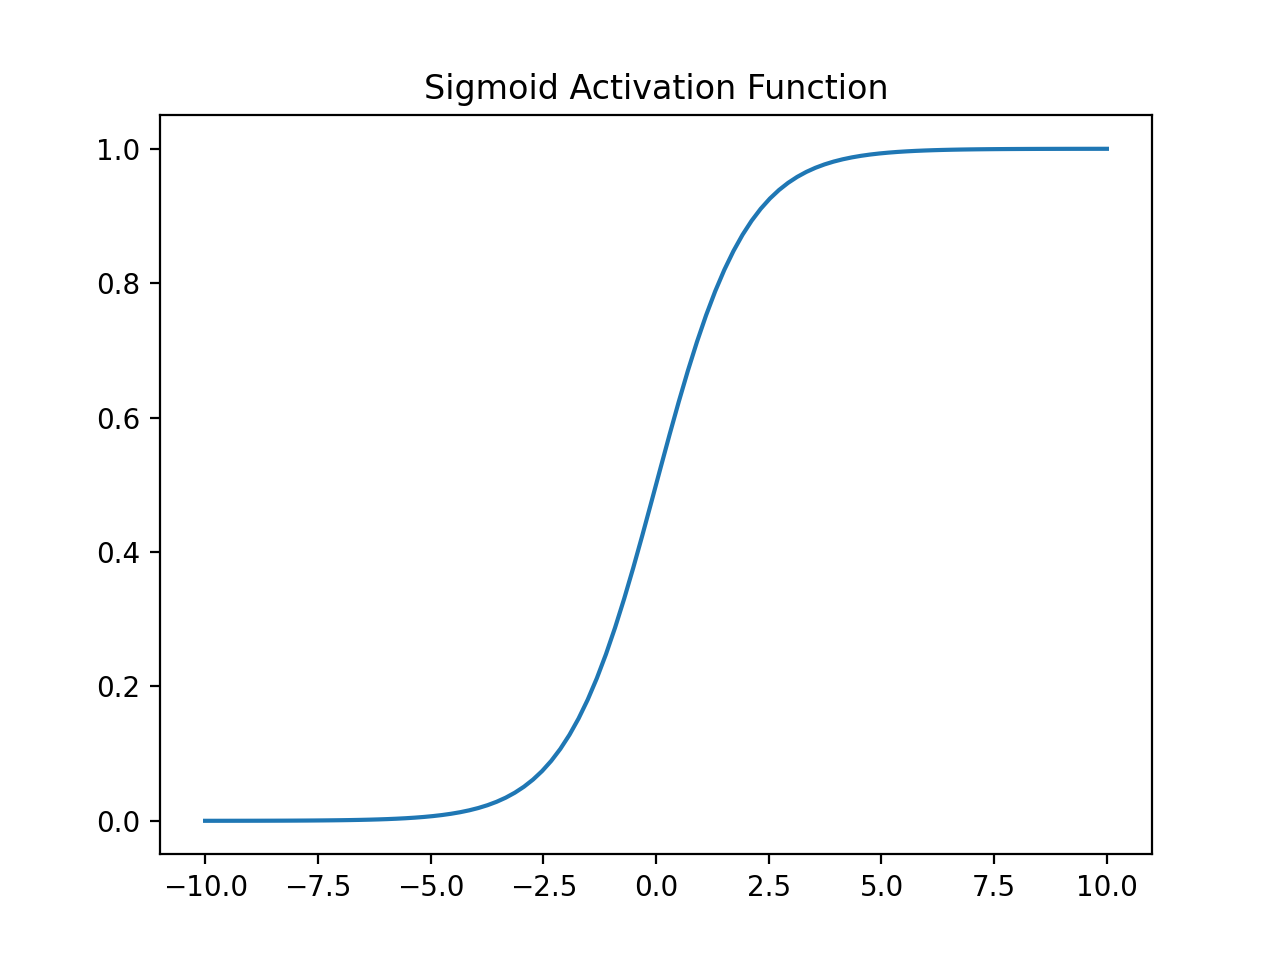
\includegraphics[width=.65\linewidth]{Images/sigmoid.png}
    \caption{Sketch of the Sigmoid Activation Function}
\end{figure}

There are three types of gates utilised within a neural network: a forget gate, an input gate, and an output gate. A forget gate decides what information should be thrown away or kept. Information from the previous hidden state and information from the current input is passed through the sigmoid function. An input gate is where the previous hidden state and current input into a sigmoid function. The output gate decides what the next hidden state should be. The hidden state is also used for predictions. First, we pass the previous hidden state and the current input into a sigmoid function. Then we pass the newly modified cell state to the rectified linear activation function. We multiply the rectified linear activation function output with the sigmoid output to decide what information the hidden state should carry. The output is the hidden state. The new cell state and the new hidden is then carried over to the next time step\cite{lstm_rnn}.

\subsection{Implementation}\label{implement_rnn}
The data set for the initial conditions (which is discussed in section \ref{noaa_initial_conditions}) consists of three features: geopotential height, air temperature, and relative humidity. For the purposes of this specific project, the RNN will solely be trained on air temperature and relative humidity. Unfortunately, due to the COVID-19, there was a time constraint on the developed of the RNN, which resulted in the inability to also train the RNN on geopotential height. This is due to the lack of computational resources at my disposable. The data set in question is updated every six hours by the National Oceanic and Atmospheric Administration. This means for a single day, there will be four observations. The goal for this project will be to, first predict the relevant atmospheric parameter in seven days time given the last thirty days of data and combine this RNN prediction with the physical model prediction in an attempt to make a more accurate prediction overall. In order to make such predictions, it is necessary to create a window of the last 120 ($30 \times 4$) observations to train the model\cite{time_series}.

At the start, a seed is set in order to ensure reproducibility. As mentioned previously, it is important to scale features before training a neural network. Normalisation is a common way of doing this scaling by subtracting the mean and dividing by the standard deviation of each feature. In order for the most optimal performance, the method ``MinMaxScaler" from the library, scikit-learn, is utilised within the software\cite{scikit-learn}. An LSTM requires a 1-dimensional sequence, however, the atmosphere is a 3-dimensional system. Hence, it is necessary to flatten the 3-dimensional vector that represents the state of the atmosphere. This is done in order to avoid the need of repeatably running the RNN. Batches are then created to split the data into manageable sequences. The diagram on the following page shows how the data is represented after flattening the data and batching it (provided by Tensorflow)\cite{time_series}.

\begin{figure}[H]
    \centering
    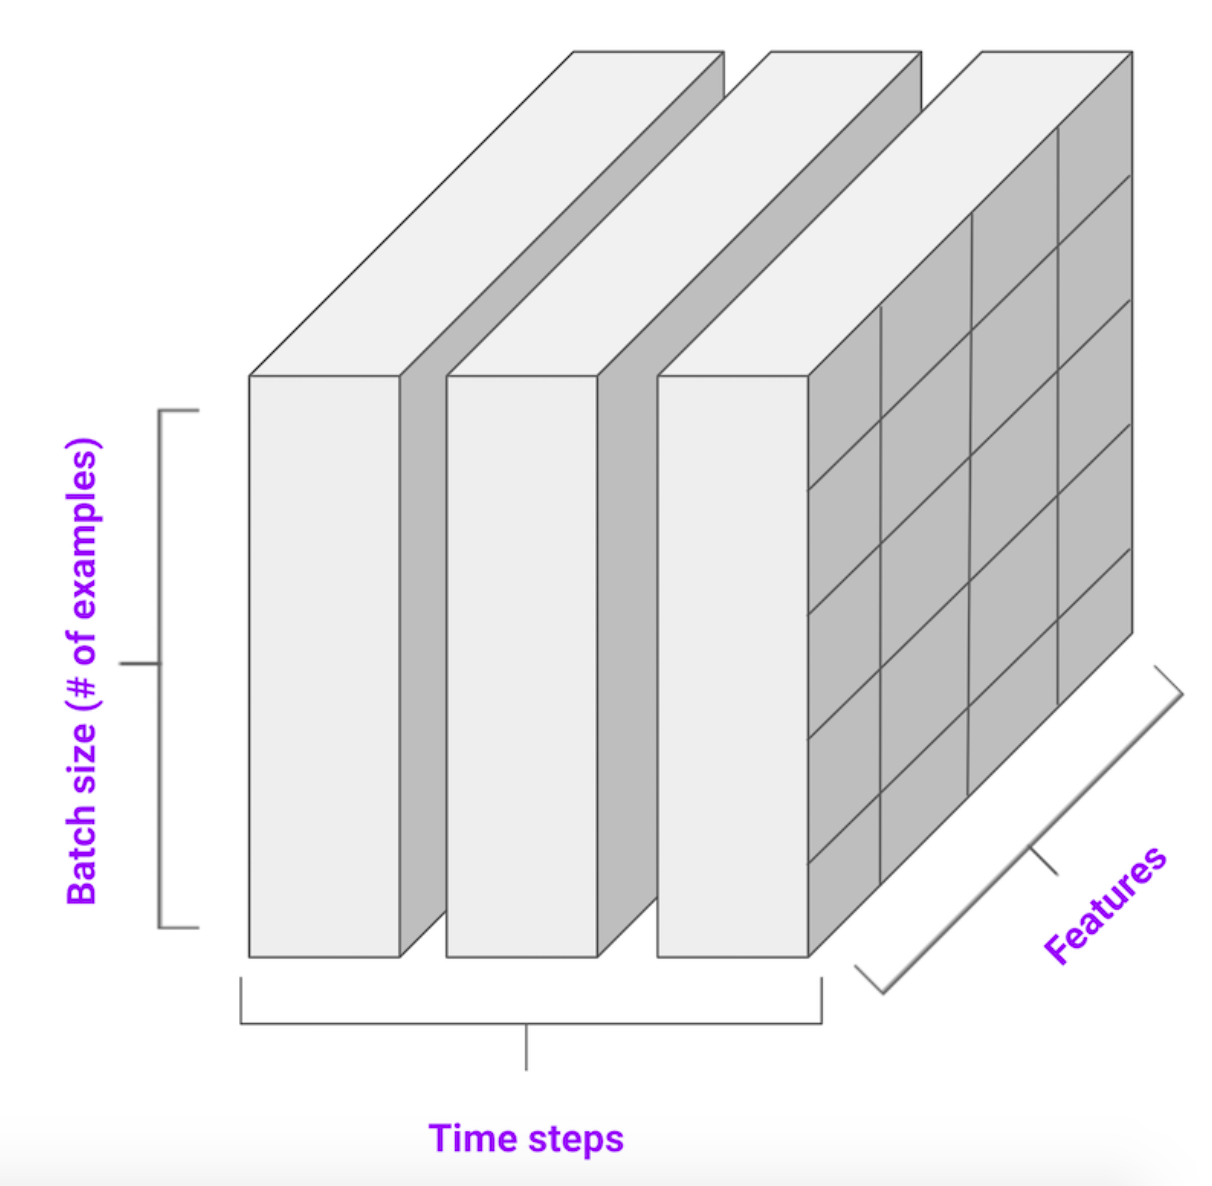
\includegraphics[width=.5\linewidth]{Images/data_rnn.png}
    \caption{Visualisation of how the data is represented after flattening and batching.}
\end{figure}

Following this process, the data is feed into the RNN. The LSTM model is built using Keras in TensorFlow, which is an free and open-source software library for machine learning. It was developed by the Google Brain Team\cite{tensorflow}. It is apparent that a multi-step model is needed as the model needs to learn to predict a range of future values. The source code for the LSTM model developed for the software is shown below:

\begin{minted}[mathescape,linenos,frame=lines]{python}
# Prepossessed historical data, which has been flatten and batched.
x_data, y_data = prepossessing_function(input_data)
# Prepossessed initial conditions, which has been flatten and batched.
initial_conditions = prepossessing_function(input_initialconditions)

# The network is shown data from the last 15 days.
past_history = 15 * 4

# The network predicts the next 7 days worth of steps.
future_target = 7 * 4

# Create, and train models.
# Optimiser.
opt = Adam(lr=1e-6, decay=1e-10, clipvalue=0.6)
# Create model.
model = Sequential()
model.add(
    LSTM(
        400, activation='relu', input_shape=(past_history, features)
    )
)
model.add(RepeatVector(future_target))
model.add(LSTM(400, activation='relu', return_sequences=True))
model.add(LSTM(400, activation='relu', return_sequences=True))
model.add(LSTM(400, activation='relu', return_sequences=True))
model.add(TimeDistributed(Dense(features)))
model.compile(
    optimizer=opt, loss='mse', metrics=['mean_absolute_error']
)

# Train.
model.fit(
    x_data, y_data, epochs=epochs, batch_size=10
)

# Predict.
future_state = model.predict(initial_conditions)
# Invert normalisation, and flattening.
future_state = inverse_prepossessing(future_state)
\end{minted}

The model consists of four LSTM layers, which in combination are able to produce a more accurate and reliable prediction than a single LSTM layer. As is evident, the activation function for each LSTM is the rectified linear activation function, which is built into Keras. The number of epochs can be specified by the end user depending on the computational resources they have and what they need. More epochs will evidently lead to a more accurate neural network.

\begin{definition}
An epoch is one forward pass and one backward pass of all the training examples.
\end{definition}

\section{Initial Conditions}\label{noaa_initial_conditions}
\subsection{Global Data Assimilation System}
The initial conditions utilised by the software are from the Global Data Assimilation System (GDAS), which is provided by the National Oceanic and Atmospheric Adminstration in the United States. The primary reason for utilising this data is that it is freely available to the general public. In an ideal world, data from the European Centre for Medium-Range Weather Forecasts would be utilised, however unfortunately, there data is not freely available to the general public. This fundamentally violates the software's open source principles (these principles are discussed in chapter \ref{5}).

The GDAS is a model to place observations into a gridded model space for the purpose of initialising weather forecasts with observed data. This system is utilised by the National Center for Environmental Prediction for such a purpose. GDAS adds the following types of observations to a gridded, 3-D, model space: surface observations, balloon data, wind profiler data, aircraft reports, buoy observations, radar observations, and satellite observations\cite{gdas}. The initial conditions provided by the GDAS to the software have a vertical pressure co-ordinate, or the vertical co-ordiante is pressure. This co-ordinate system is known as isobaric co-ordinates.

\subsection{Isobaric Co-Ordinates}
In coordinate systems applied to the earth, the vertical coordinate describes position in the vertical direction (that is, parallel to the force of effective gravity). In meteorology, pressure can be a more convenient vertical coordinate than altitude. One reason is that until recently, radiosondes, which are the primary means of gathering observations of weather variables above the earth’s surface, measure and reported pressure, temperature, and humidity, but not altitude, as they rise through the atmosphere\cite{isobar_i}.

\begin{definition}
A radiosonde is an instrument carried by balloon to various levels of the atmosphere and transmitting measurements by radio.
\end{definition}

Another reason is that on scales large enough for the hydrostatic approximation to be valid (this is discussed in section \ref{hydro_balance}), the pressure-gradient force in the equations of motion becomes simpler and density no longer becomes an explicit variable in the tendency equations\cite{isobar_i}. Thus,a given geopotential gradient implies the same geostrophic wind at any height, whereas a given horizontal pressure gradient implies different values of the geostrophic wind depending on the density\cite{isobar_ii}.

From the Global Data Assimilation System, three prognostic variables are chosen: geopotential height, air temperature, and relative humidity.

\begin{definition}
Geopotential Height is the height above sea level of a pressure level. For example, if a station reports that the 500 hPa height at its location is 5600 m, it means that the level of the atmosphere over that station at which the atmospheric pressure is 500 hPa is 5600 meters above sea level.
\end{definition}

Geophysical sciences such as meteorology often prefer to express the horizontal pressure gradient force as the gradient of geopotential along a constant-pressure surface, because then it has the properties of a conservative force. For example, the primitive equations which weather forecast models solve use hydrostatic pressure as a vertical coordinate, and express the slopes of those pressure surfaces in terms of geopotential height. As such, this will be a parameter of great interest. From the aforementioned three selected parameters, any other parameter that is needed in the software can be calculated, including the wind. This will be discussed in greater depth in the next chapter.  
